\documentclass[10pt,journal,a4paper]{IEEEtran}
\usepackage{tikz}
\usepackage{amsmath}
\usepackage{amssymb}
\usepackage{graphicx}
\usepackage{caption}
\usepackage{cleveref}
\usepackage{subcaption}

\begin{document}
%
% paper title
% can use linebreaks \\ within to get better formatting as desired
\title{NOOC Paper Review\\Gossip vs. Markov Chains}
\author{\begin{tabular}{rl}
\textbf{Jean-Baptiste Cordonnier}&\texttt{jean-baptiste.cordonnier@epfl.ch}\\\textbf{Ismail Bouanani}&\texttt{ismail.bouanani@epfl.ch}
\end{tabular}}

\IEEEcompsoctitleabstractindextext{
\begin{abstract}
Rumor spreading is a well known problem with multiple applications, from information broadcast in complex distributed systems to analysis of viral content on social networks. This project report will go over the paper of Guo and Sun \cite{guosun} analyzing the natural rumor spreading algorithm using random walks and Markov chains. We aim at providing a good understanding of the mathematical tool and  the concepts used to show that the number of time steps needed to spread a rumor is $O(\log n)$. This report also study one of the main concerns: the randomness requirement needed to run the algorithm. We will finally provide simulation of this algorithm on specific graphs. 
\end{abstract}
}

\newcommand{\norm}[1]{\left\lVert#1\right\rVert}
\newtheorem{theorem}{Theorem}
\newtheorem{definition}{Definition}
\renewcommand{\l}{\left}
\renewcommand{\r}{\right}
\renewcommand{\P}[1]{\mathbf{P}\l\{#1\r\}}
\newcommand{\E}[1]{\mathbf{E}\l[#1\r]}

% make the title area
\maketitle
\IEEEdisplaynotcompsoctitleabstractindextext

\section{Introduction}

In any distributed information system it is a common task to share a piece of information with other nodes of the system. This task can be seen as spreading a rumor across a graph of connected nodes form a source vertex. At each time step any informed node can reach out to one of his neighbor until all the nodes are informed. The rumor spreading protocol is the simplest algorithm we can come with in order to solve the rumor spreading problem. Given a starting node $s$ (the source of the gossip), we keep track of a set of informed nodes $S$. At each time step of the algorithm, each informed node selects one of his neighbor uniformly at random and inform him. Step after step the set of informed nodes will grow until it contains all the vertex of $G$. Once a node is informed he becomes an informer and will spread the gossip during the upcoming time steps.

This rumor spreading protocol has been extensively studied and the $O(\log n)$ bound is well known (with $n$ being the number of nodes). This paper comes after a serie of papers proving this bound in different set-up with diverse assumptions on the graph (regularity, diameter, conductance). This paper uses a new technique of simulating the push and pull of the rumor with forward and backward random walks, it yields the following main result:

\vspace{.3cm}
\noindent\fbox{\begin{minipage}{0.97\linewidth}
\textbf{Main result.}
  Let $G$ be a graph with $n$ nodes, spectral gap $\alpha$ and irregularity $\beta$. Then there is an explicit protocol using $O(C \log n) + \tilde O(\log n)$ random bits, where $C=(\log (1/\alpha) + \log \beta)$ such that with high probability all nodes get the rumor in $T=O(C' \log n)$ rounds, where $C' = (1/\alpha) \cdot \beta^2 \max(1, 1/(\alpha \cdot \Delta ^ {0.499}))$
\end{minipage}}
\vspace{.3cm}

The intuition behind any case of rumor spreading is that the topology of the graph has a great impact on the efficiency of our algorithm. For instance, nodes very poorly connected and far from the center are hard to reach and terrible rumor sources. This essence of "good" and "bad" graphs is captured by the spectral gap $\alpha$ and the irregularity $\beta$. The spectral gap $\alpha$ is defined by $\alpha \triangleq 1 - \lambda_2$ where $\lambda_2$ is the second eigenvalue of the Laplacian matrix associated to the graph \cite{jerrum} and is related to the graph conductance. Intuition tells us that if there are a lot of edges and no bottleneck then the flow should spread out quickly and the Markov chains mix rapidly. The irregularity $\beta$ is defined as $\beta \triangleq \Delta/\delta$ (highest over lowest node degree) and captures the heterogeneity of the node degrees. If the graph is  irregular, a very isolated source node could be picked as the source of the gossip and it would take more time to inform all the network.

\textbf{TODO: add a word on randomness}

\section{Proof outline}

The analysis in the paper of Guo and Sun \cite{guosun} compares the problem of gossip spreading to many random walks in parallel. At each round, a random walk take a step on a graph as the rumor would spread between the nodes. Whenever a node $u$ pushes the information to an uninformed node $v$, one random walk stays in $u$ and another one goes to $v$. The random walk that "stays" in the same node is called $lazy$ while the other one is non-lazy (or $\overline{lazy}$). This split of random walks characterize the fact that the information is now present both in $u$ and $v$. Node $u$ will continue to spread the knowledge in the following rounds.

The main idea behind the proof is to use the duality of information sharing. Whenever a node $u$ informs $v$, we say that he pushes the information to $v$ but we can also consider that $v$ pulled the information from $u$. We then define two types of random walks when the information is spread through the graph: forward and backward random walks. Forward random walks start from the source $s$ and are pushing the information through a path while the backward random walks start from a targeted node $t$ and pull the information. For instance, if a node $u$ pushes information to a node $v$, a forward random walk would take a step from $u$ to $v$ and a backward random walk would take a step from $v$ to $u$, that remains true if and only if $u$ is the only node that pushed to $v$ is $u$. In practice there is no way for a node to pull the information as long as no neighbor is informed, that's why the backward random walks are only used for the analysis. Finally, to know if a target node $t$ has been informed, we only need to know if there exists a node $v$ reached by a forward random walk from $s$ and by a backward random walk from $t$.


\begin{figure}[h]
\centering
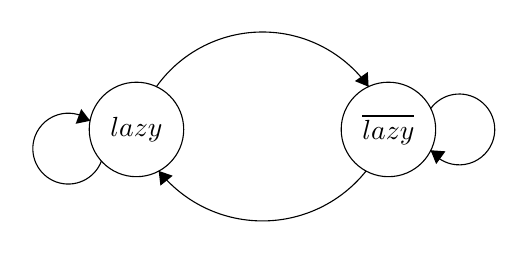
\begin{tikzpicture}[scale=0.2]
\tikzstyle{every node}+=[inner sep=0pt]
\draw [black] (26.1,-26.6) circle (3);
\draw (26.1,-26.6) node {$lazy$};
\draw [black] (42.1,-26.6) circle (3);
\draw (42.1,-26.6) node {$\overline{lazy}$};
\draw [black] (40.688,-29.229) arc (-38.4609:-141.5391:8.413);
\fill [black] (27.51,-29.23) -- (27.62,-30.17) -- (28.4,-29.54);
\draw [black] (27.358,-23.895) arc (144.65362:35.34638:8.265);
\fill [black] (40.84,-23.89) -- (40.79,-22.95) -- (39.97,-23.53);
\draw [black] (23.878,-28.598) arc (-20.31276:-308.31276:2.25);
\fill [black] (23.16,-26.05) -- (22.59,-25.3) -- (22.24,-26.24);
\draw [black] (44.78,-25.277) arc (144:-144:2.25);
\fill [black] (44.78,-27.92) -- (45.13,-28.8) -- (45.72,-27.99);
\end{tikzpicture}
\caption{Random walk state}
\label{fig:lazyFSM}
\end{figure}

To show that any node $w$ will be reached after a given number of rounds we consider all the possible spreading path from the source $s$. The information reaches $w$ as long as there is an intermediary node $u$between a forward random walk from $s$ and a backward random walk from $w$ as explained earlier. To set the lower bound, we consider all the random walks pattern after $k$ steps $S \in \mathcal C_k = \{ lazy, \overline{lazy} \}^k$ as in \cref{fig:lazyFSM}. Let's define the indicator random variable $X_{u,v}^S$ (resp. $Y_{u,v}^S$) that the forward (resp. backward) random walk with pattern $S$ and initial node $u$ ends up at node $v$. To show that a node $w$ is reached by the gossip in $T$ steps we need to find a vertex $u$ such that $X_{s,u}^{S}Y_{w,u}^{S'} = 1$ with $S, S' \in \mathcal C_{T/2}$. We can now lower bound the probability of a node to be informed in $T$ steps as follow
\begin{align*}
  \scriptsize
  \P{w \text{ informed in $T$ rounds}} \geq \P{\sum_{S,S'\in \mathcal C_{T/2}, u\in V[G]} X_{s,u}^S Y_{w,u}^{S'} > 0}
\end{align*}

The authors of the paper analyze this lower bound thanks to random walks taken individually and pair wisely. The need to analyze two random walks together to get a lower bound of the expectation leads us to use Markov chain coupling. Formally, a matrix coupling is defined as follow:

\begin{definition}
  A stochastic matrix $\mathbf{M'' \in \mathbb{R}^{n\times n} \otimes \mathbb{R}^{n\times n}}$ is a coupling of $\mathbf{M,M''} \in \mathbb{R}^{n\times n}$ if $\sum_{x\in[n]} \mathbf{M''}_{(u,w)(v,x)} = \mathbf{M}_{u,v}$ for any $u,w,v \in [n]$ and $\sum_{v\in[n]} \mathbf{M''}_{(u,w)(v,x)} = \mathbf{M'}_{w,x}$.
\end{definition}

The intuition behind this is that we are mixing two Markov chains together and coupling their state. Now the state of $\mathbf{M''}$ will contain the state of both Markov chains, and the two Markov chains will behave independently according to their own transition distributions. The paper \cite{guosun} also defines lazy Markov chain with a slack parameter $\gamma$ that represents the probability for a Markov chain to stay idle at the same state (by increasing the diagonal probabilities):

\[
  \mathcal L _ \gamma (\mathbf{M}) \triangleq (1-\gamma) \mathbf{I} + \gamma \mathbf{M}
\]

We similarly define a lazy coupling of $\mathbf{M}$ and $\mathbf{M'}$ noted $\mathcal L_{\gamma, \gamma'}(\mathbf{M''})$ to be the coupling of $\mathcal L_\gamma(\mathbf{M})$ and $\mathcal L_{\gamma'}(\mathbf{M'})$. The last tool needed to characterize our bound with Markov chain is the Doeblin coupling \cite{coupling}. It reflects the fact that when two random walks are at the same node $u$ at the same time step $t$, they will stay together for all the remaining steps because the node $u$ can push the information to a single node $v$ chosen uniformly and both random walks (if non-lazy) should go to the same node. The Doeblin coupling of two copies of $\mathbf{M}$ is formally expressed as

\[
  \mathcal Q(\mathbf{M})_{(u,w)(v,x)} \triangleq \left\{
    \begin{array}{ll}
      (\mathbf{M} \otimes \mathbf{M})_{(u,w)(v,x)} & u \not = v,\\
      \mathbf{M}_{(u,v)} \cdot \mathbf{1}_{v = x} & u = v.\\
    \end{array}
  \right.
\]

The aim of this lemma is to show that after $k$ rounds, and independently of the pattern followed (we consider the lazy version of the matrix here), any distribution is identical to the stationary distribution $\pi \otimes \pi$ (i.e $P(u,v)=(1/n)^2$) for all $(u,v) \in V[G] \times V[G]$. To do so, we lower bound the quadratic distance

\[
  \norm{u(\mathcal L_{\gamma,\gamma} \circ \mathcal Q(M))^k - \pi \otimes \pi}_2 \leq (1 - \gamma \alpha / 2)^k + 2 \sqrt 2 \gamma \alpha^{-1} n^{-3/2}
\]

\textbf{TODO: expander graph}

The conclusion for that is, the convergence of the process does not depend on the node who has the information first since after $k$ rounds ($k$ big enough), the parallel $2^k$ Markov chains have joint evolutions (or almost).

A drawback for that protocol would be its consumption of too many random bits which is O(n logn) per round. Indeed, at each round ,each informed node (worst case n in total) fills a log n-long bit string to define the neighbor receiving the information.

\section{Randomness requirement}

One common thing about all  the protocols below is that in all of them we seek for randomness and efficiency. Randomness means that the rumor spreading is independent on the first node that has the information.It also means that the choice of the node an informed node transmits the  information to is close to a uniform choice among its adjacency list (actually is uniform in the first protocol). Efficiency means that the rumor is spread all over the network almost surely in a number of rounds $T=O(\log n)$, our results say that it is the case. In addition to that, efficiency means we want to generate as few random bits as possible, at that level some are better than the others, we will get to it.

In order to reduce the cost of the protocol in terms of random bits, a different protocol with a different way to chose the neighbor is designed. The second protocol uses pseudo-random generators,one for seed length $l'$ that produces $T/2 $ l-bits outputs (one for each round). Concretely, it means, for a given node, it is a way to determine to which neighbor the information will be transmitted. Roughly speaking, pseudo-randomness means $P(G’0(x)=\underbrace{0\dots0}_l)$ for a $l’$-length seed $x$ for instance is equal to $(1/2)^l$ (approximatively). We also use a pseudo random generator $f$:$l$-bits word $\to$ an index modulo delta for each possible node. To sum things up, all the randomness lie in the l’ bits seed that the system generates (actually there are two of them), then for each round the $G’$ PRG assigns a l bits word to these seeds ($x$ if round before $T/2$ and $y$ otherwise). From this $l$ bits word, each informed node generates an index to modulate according to its neighbor list to know which neighbor to inform.
 The method to follow, is to start from arbitrary $l’$-long bit strings $x,y$. Construct a pseudo random generator
  \[
    ( \zeta'_{0}, \dots, \zeta'_{T/2}): \{ 0,1 \}^{l'} \to ( \{0,1\}^T/2 )
   \]
 
for branching process $(T/2,n^2,2^l)$. The theorem D.5 tells us that $l=O(\log m+\log n)$ where $m=n^{\theta(1)}$,thus $l=O(\log(n^2))$. Then, we contract a pseudo random generator for CRs where $s=[m]^n$ with $m=n^{\theta(1)}$, we then apply the protocol described. One can notice that the seed length l’ is in O(log n). That would be because it is supposed to represent a random node on the whole n-nodes graph, which is coded in O(log n) bits.
 
We now present two other random protocols following the same principle of informing one neighbor (thus still in $T=O(C^*\log n)$) but that cost much less random bits. We start from a random $l$ bits seed. Each node has an identity once it is informed, with this feature, we can say from a node's ID in which round it has been informed.The neighbor index is chosen at random through an expander function and a pseudo-random generator. We say this protocol uses $O(\log\log n + \log \delta)$ random bits per round because it generates from the seed at most M blocks, the size of adjacency list of the most connected informed node at the round and $M=O(D)=O(\log n / \epsilon)=O(\delta^*\log n)$ since $\epsilon=\delta^{-\theta(1)}$. To encode it, we need $O(\log\log n + \log \delta)$ random bits. Once we generated the blocks, the expander function computes for each informed node the index of the block that corresponds to the node to inform. This protocol is clearly less expensive than the second one, that uses $O(\log n)$ random bits per round (generates one block per informed node so $O(n)$ blocks). The other one uses the same tools but with different parameters, it is adaptable to expander graphs. An expander graph is a graph that has small irregularity and a spectral gap close to 1, so it is strongly connected, almost $d-$regular $d=O(\delta)$. It is,according to the paper the worst case scenario for which the process converges slow.
 

\section{Simulations}

To illustrate our initial intuition about what makes a graph "good" or "bad" for rumor spreading, we made some simulation of the rumor spreading protocol on different generated graphs. Our first goal was to run the algorithm on a model as close as possible to social graphs. We started with the simplest model that we have seen in class, the $C(n,p)$ graphs. Later, we found that the Barabasi-Albert graph model \cite{abmodel} have properties much closer to real life network and we ran the protocol on it. This model is more realistic of how real networks look like with important hub and preferential attachment for already well connected nodes (i.e. popular person on social medias). Also the clustering coefficients of Barabasi-Albert model are known to be much higher than for random graphs. The figures \ref{barabasi-albert-graphs} show the evolution of a rumor in such a graph. The beginning of the spreading is quite slow because very few nodes have the information, then it grows exponentially fast before slowing down because very few nodes are left to be informed. 

\begin{figure}[h]
\centering

\begin{subfigure}[b]{.5\linewidth}
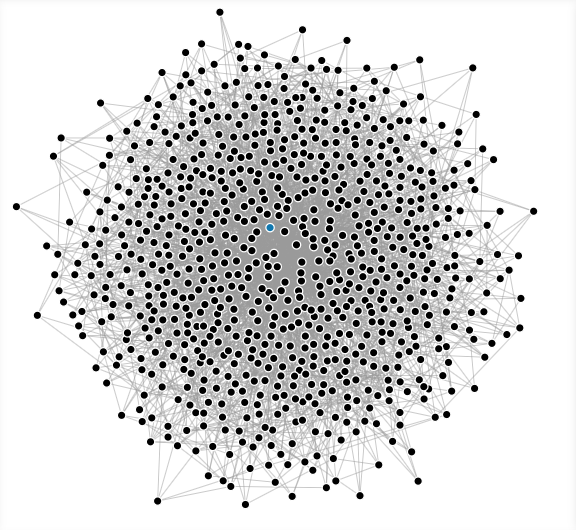
\includegraphics[width=1\linewidth]{figs/barabasi-albert-0}
\caption{$T=0$}
\end{subfigure}%
\begin{subfigure}[b]{.5\linewidth}
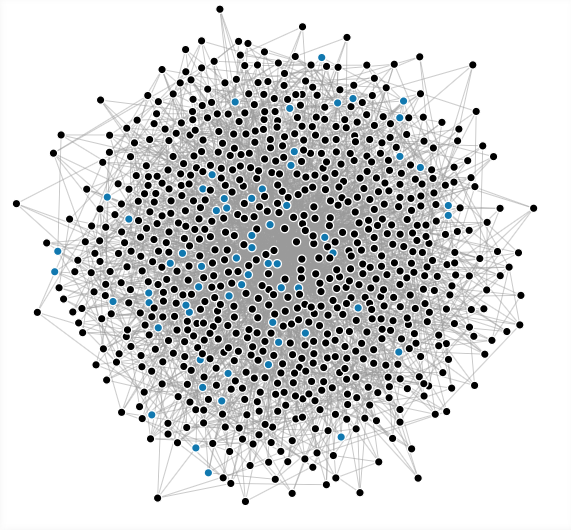
\includegraphics[width=1\linewidth]{figs/barabasi-albert-4}
\caption{$T=4$}
\end{subfigure}

\begin{subfigure}[b]{.5\linewidth}
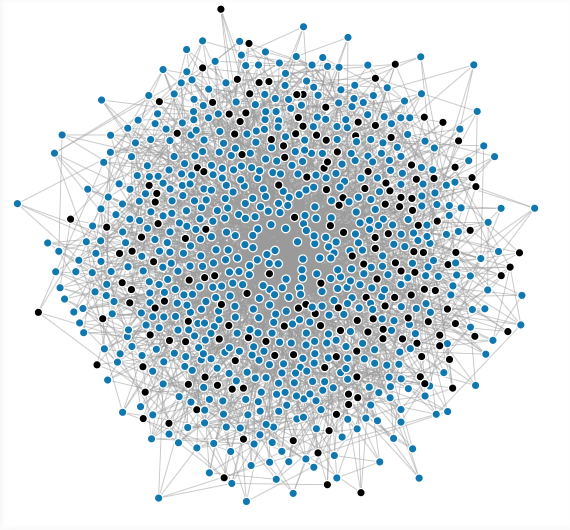
\includegraphics[width=1\linewidth]{figs/barabasi-albert-8}
\caption{$T=8$}
\end{subfigure}%
\begin{subfigure}[b]{.5\linewidth}
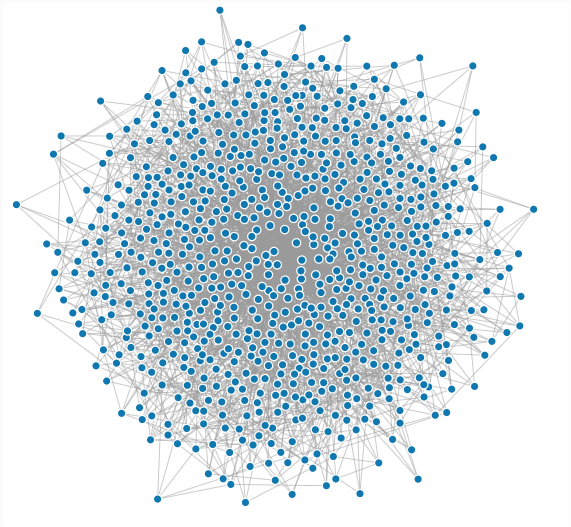
\includegraphics[width=1\linewidth]{figs/barabasi-albert-12}
\caption{$T=12$}
\end{subfigure}

\caption{Rumor spreading (blue nodes) in Barabasi Albert graph with $n=800$, $m_0 = 20$ and $M = 4$}
\label{barabasi-albert-graphs}
\end{figure}

\begin{figure}[h]
\centering
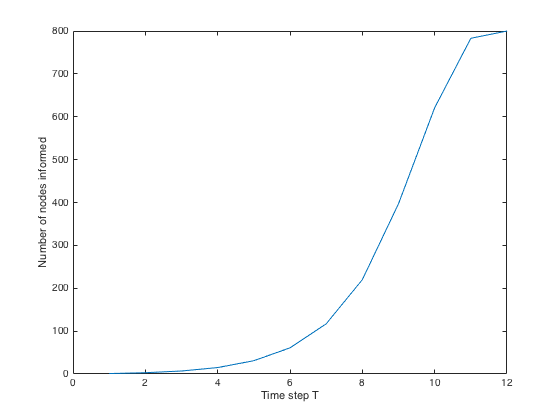
\includegraphics[width=1\linewidth]{figs/barabasi-albert-chart}
\caption{Number of nodes informed over time in the Barabasi Albert simulation}
\label{fig:barabasi-albert-chart}
\end{figure}

It is more interesting to study malformed graphs where some nodes are hard to reach. We take an simple example of a graph composed of two distinct graphs $C(n,p)$ with very few connections between the two, these connections are picked  uniformly and independently with probability $q$ ($q << p$). These edges will form a bottle neck harder to cross for the gossip and the two distinct populations will struggle to share any information. Given that this bottle neck is a good cut, this graph has a very low conductance and the constant in the $\log n$ is affected badly. 

\begin{figure}[h]
\centering

\begin{subfigure}[b]{.5\linewidth}
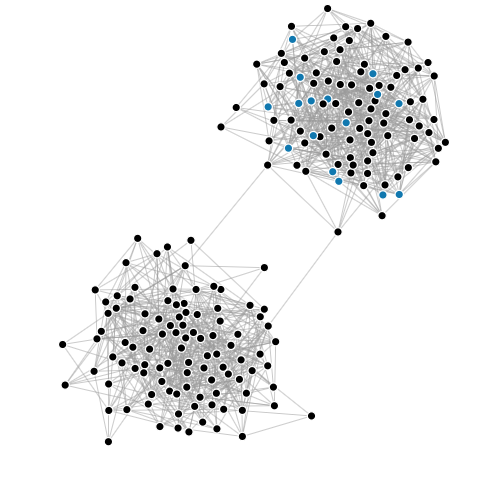
\includegraphics[width=1\linewidth]{figs/split-1}
\caption{$T=3$}
\end{subfigure}%
\begin{subfigure}[b]{.5\linewidth}
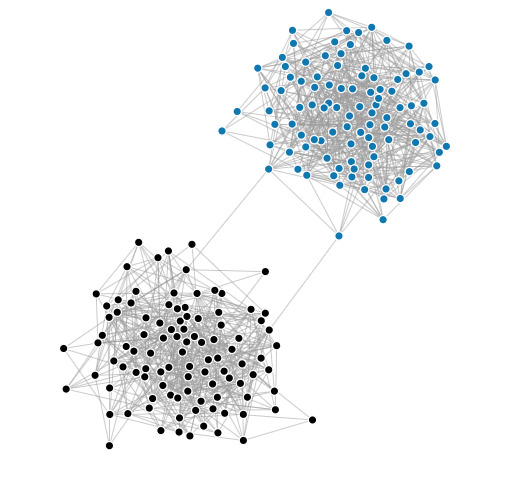
\includegraphics[width=1\linewidth]{figs/split-2}
\caption{$T=9$}
\end{subfigure}

\begin{subfigure}[b]{.5\linewidth}
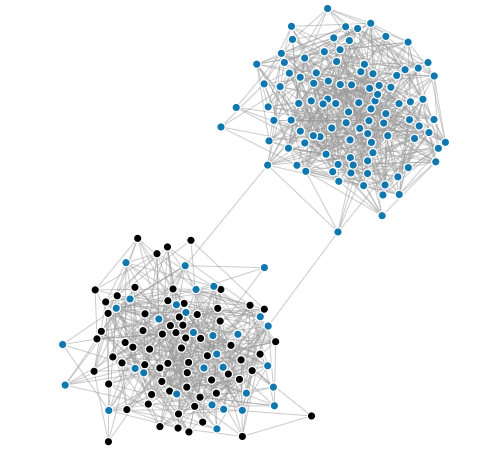
\includegraphics[width=1\linewidth]{figs/split-3}
\caption{$T=13$}
\end{subfigure}%
\begin{subfigure}[b]{.5\linewidth}
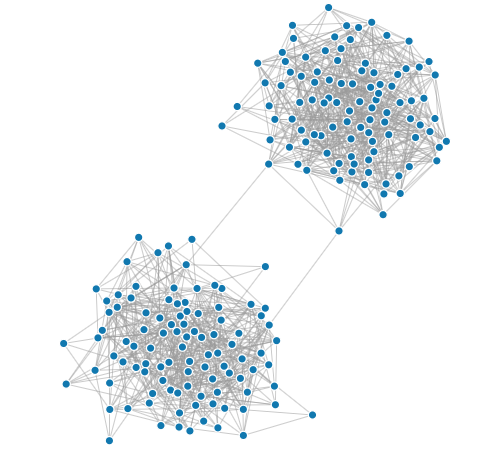
\includegraphics[width=1\linewidth]{figs/split-4}
\caption{$T=17$}
\end{subfigure}

\caption{Rumor spreading (blue nodes) in bottleneck model with $n=100$, $p = 0.1$ and $q = 0.0003$}
\label{barabasi-albert-graphs}
\end{figure}


\begin{figure}[h]
\centering
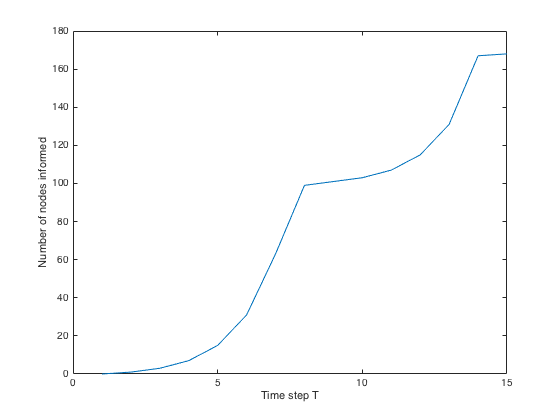
\includegraphics[width=1\linewidth]{figs/split-chart}
\caption{Number of nodes informed over time in the bottleneck simulation}
\label{fig:split-chart}
\end{figure}

We can see in \cref{fig:split-chart} that the number of informed nodes palliates when the rumor has to cross the bottleneck. It is normal that the topology of a network affects the quality of the broadcast and bridging an information between two very well distinct populations is hard. The experimental value of $\lambda_2$ is $0.9936$ which gives a very small $\alpha$ and $1/\alpha = 156.3$ still we can see an exponential trend but the constant depending on $1/\alpha$ and will make the spread much slower.

\begin{table}
\centering
\begin{tabular}{c|c|c||c|c|c}
  $q (10^{-5})$ & \# crossing & $\alpha (10^{-4})$ & .5 & .9 & 1\\
  \hline
  1 & 8 & 1.5 & 13 & 21 & 22 \\
1.3 & 15 & 2.9 & 13 & 20 & 21 \\
1.7 & 28 & 5.5 & 13 & 19 & 20 \\
2.2 & 18 & 3.5 & 13 & 20 & 21 \\
2.8 & 33 & 6.4 & 13 & 19 & 20 \\
3.6 & 43 & 8.4 & 13 & 18 & 20 \\
4.6 & 51 & 10.0 & 13 & 18 & 20 \\
6.0 & 57 & 11.2 & 13 & 18 & 19 \\
7.7 & 73 & 14.2 & 13 & 18 & 19 \\
10 & 129 & 25.2 & 13 & 17 & 18 \\
\end{tabular}
\caption{Quantiles of the proportion of informed node during rumor spreading protocol on a bottle neck graph with bridging probability $q$, $n = 2 \cdot 1000$ and $p = 0.1$}
\label{tab:quantiles}
\end{table}

We then simulate a range of bottle neck graphs for different parameters $q$ which are summarized in \cref{tab:quantiles}. The number of crossing edges is the smallest cut of the graph and is linked to $\alpha$. The lower the number of crossing edge is, the harder it is to make the bridge between the two populations and then it is consistent that the protocol takes more iteration to inform all the nodes. Indeed $1/\alpha$ is higher when the bottle neck is tighter and the number of rounds should increase. 

\section{Conclusion}
 We have studied and analyzed different rumor spreading protocols that terminate in O(log n) rounds which can be useful for large infrastructure networks. Although those protocols are representative of real life broadcast in mobile networks (one node transmits information to one random adjacent node), we can find some weaknesses when it comes to represent social networks rumor spreading. There are two reasons for that, the first one is that in a social network like Facebook, an information can be (and most likely is) transmitted to many friends at once and not one per round. The second reason is that the node that receives the information can’t be chosen at random but in a very biased way where links have to be weighted (I share rumor with my closest friends ).However,those protocols remain the easiest ones to compute.
\begin{thebibliography}{1}

\bibitem{guosun}
Z.~Guo, H.~Sun, 
\emph{Gossip vs. Markov Chains, and Randomness-Efficient Rumor Spreading}.\hskip 1em plus
0.5em minus 0.4em\relax Proceedings of the Twenty-Sixth Annual ACM-SIAM Symposium on Discrete Algorithms, SODA 2015, San Diego, CA, USA, January 4-6, 2015.

\bibitem{jerrum}
M.~Jerrum, A.~Sinclair, 
\emph{Conductance and the rapid mixing property for Markov chains: the approximation of permanent resolved}.\hskip 1em plus
0.5em minus 0.4em\relax Proceedings of the twentieth annual ACM symposium on Theory of computing.

\bibitem{coupling}
T.~Lindvall, 
\emph{Lectures on the Coupling Method}.\hskip 1em plus
0.5em minus 0.4em\relax New York, 2002.

\bibitem{abmodel}
R.~Albert, A.-L.~Barabási 
\emph{Statistical mechanics of complex networks}.\hskip 1em plus
0.5em minus 0.4em\relax Reviews of modern physics, 2002.

\end{thebibliography}

\end{document}


